\section{Methodology}
\label{meth}

This analysis addresses the availability and overall estimated value of behind-the-meter (BTM), front-of-the-meter (FOM) and utility-scale wind throughout the state of New York. In this analysis, whether a wind turbine was deployed as BTM, FOM or utility-scale is referred to as its `application'. This analysis considered a range of turbine classes (sizes and hub heights) available for deployment, although some turbine classes were considered too small or too large for certain applications. In addition to size constraints, the eligibility for certain applications was influenced by characteristics of the parcel of land on which the turbine would be deployed. These characteristics include: available parcel land area, canopy cover, and land-use type. Once a turbine's siting, sizing and application eligibility had been determined, its generation was determined using wind resource data and power curves. Finally, given the turbine's generation, application and location within a utility territory and load zone, the appropriate values from the VDER framework were calculated.


The following sections address: 
	\begin{itemize}
		\item how wind turbines were sited within New York, including which metrics were used to determine siting availability; 
		\item how the sizes of the wind turbines were determined; 
		\item how generation profiles for the wind turbines were determined; 
		\item how costs associated with building, maintaining and operating the systems were determined; and 
		\item how values from the VDER framework were ultimately derived.
	\end{itemize}

\subsection{Turbine Siting}
\label{meth_siting}

This analysis takes advantage of an exceedingly granular, proprietary parcel-level data set referred to throughout this report as the CoreLogics data set. \hl{`Parcel-level' refers to the fact that the minimum unit under consideration for siting a wind turbine were individual parcels as opposed to states, census blocks or zip code areas.} The granluarity of this data set can be seen in Figure~\ref{fig:parcelview}. 

% creating side-by-side images out of individual images (maintains individual captioning ability), not compatible with 'conditional images'
%\begin{conditionalfigure}[!htb]
	\begin{figure}[!htb]
		\centering
			\begin{minipage}{0.3\textwidth}
				\centering
				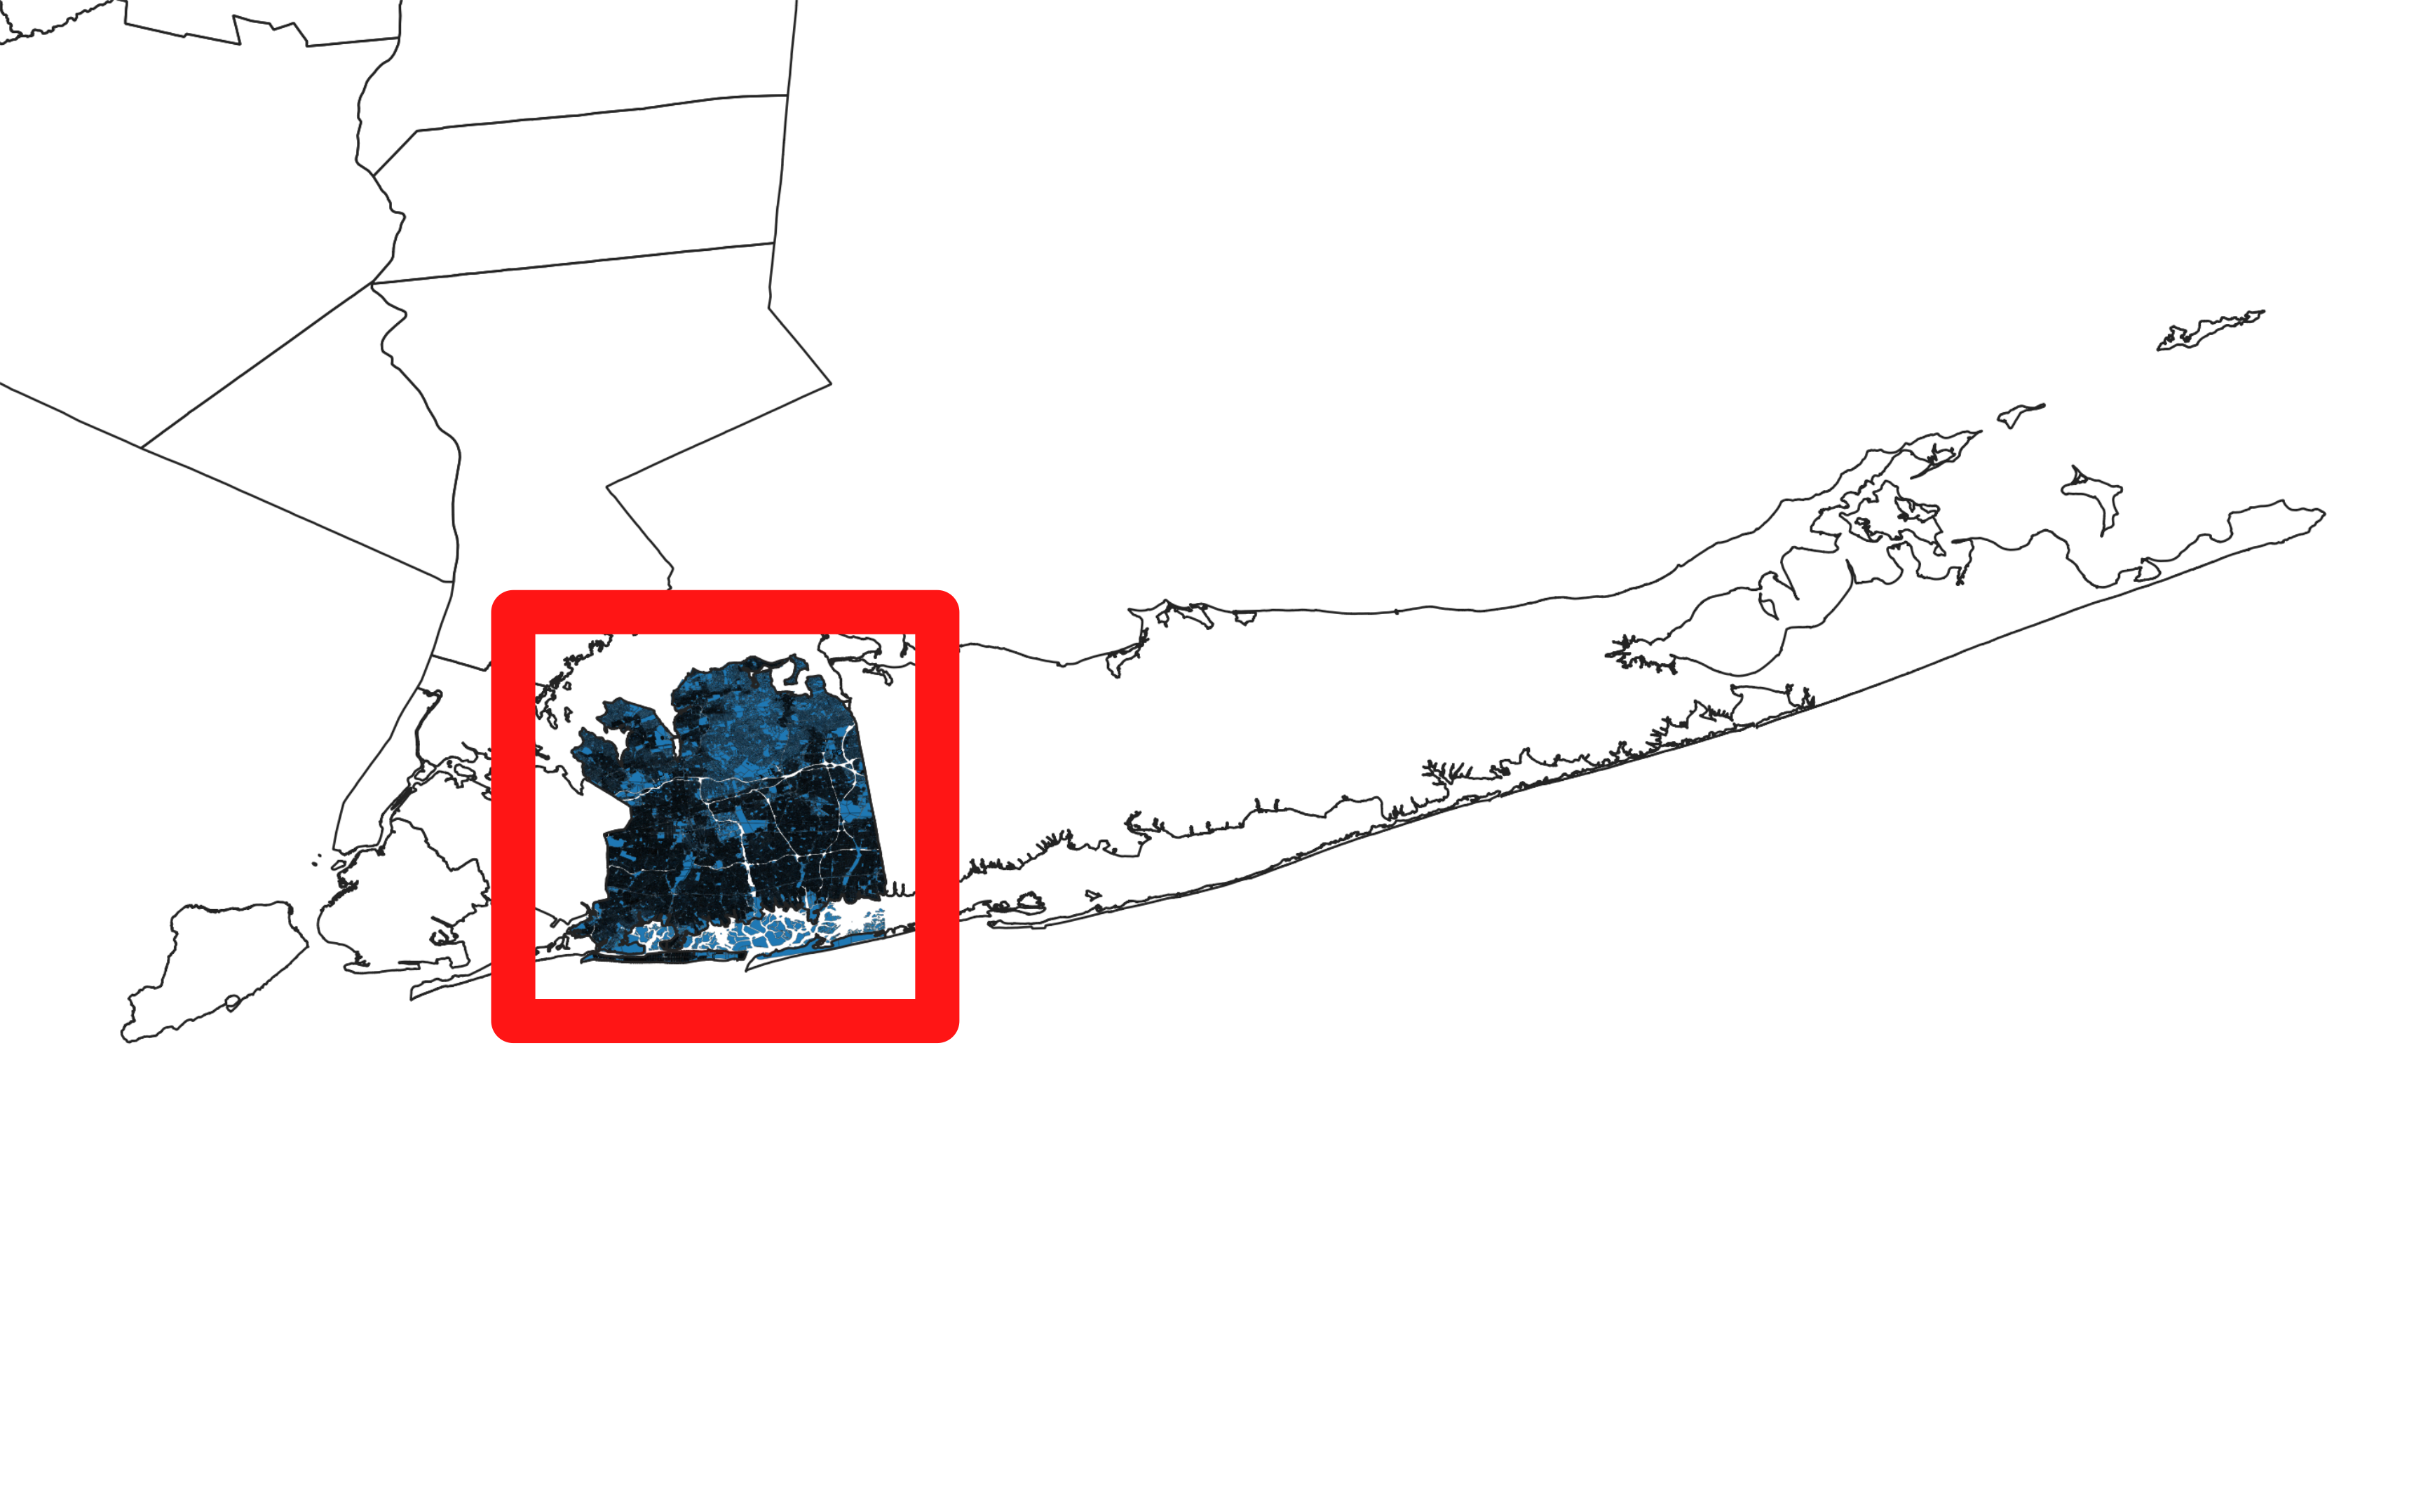
\includegraphics[width=0.9\textwidth]{parcel_dataset_images/long_island_zoomout_rev} % first figure itself
%				\caption{Zoomed-out view of Long Island}	% captions look odd for side by side figures and don't allow a 'combo caption at the bottom, better to manually fake captions for individual images and use caption for whole thing
				\footnotesize (a) Zoomed-out view of Long Island
			\end{minipage}\hfill
			\begin{minipage}{0.3\textwidth}
				\centering
				\includegraphics[width=0.9\textwidth]{parcel_dataset_images/cty_level_lowres_rev} % second figure itself
%				\caption{Zoomed-in view of Portion of Long Island}
				\footnotesize (b) Zoomed-in view of Portion of Long Island		
			\end{minipage}\hfill
			\begin{minipage}{0.3\textwidth}
				\centering
				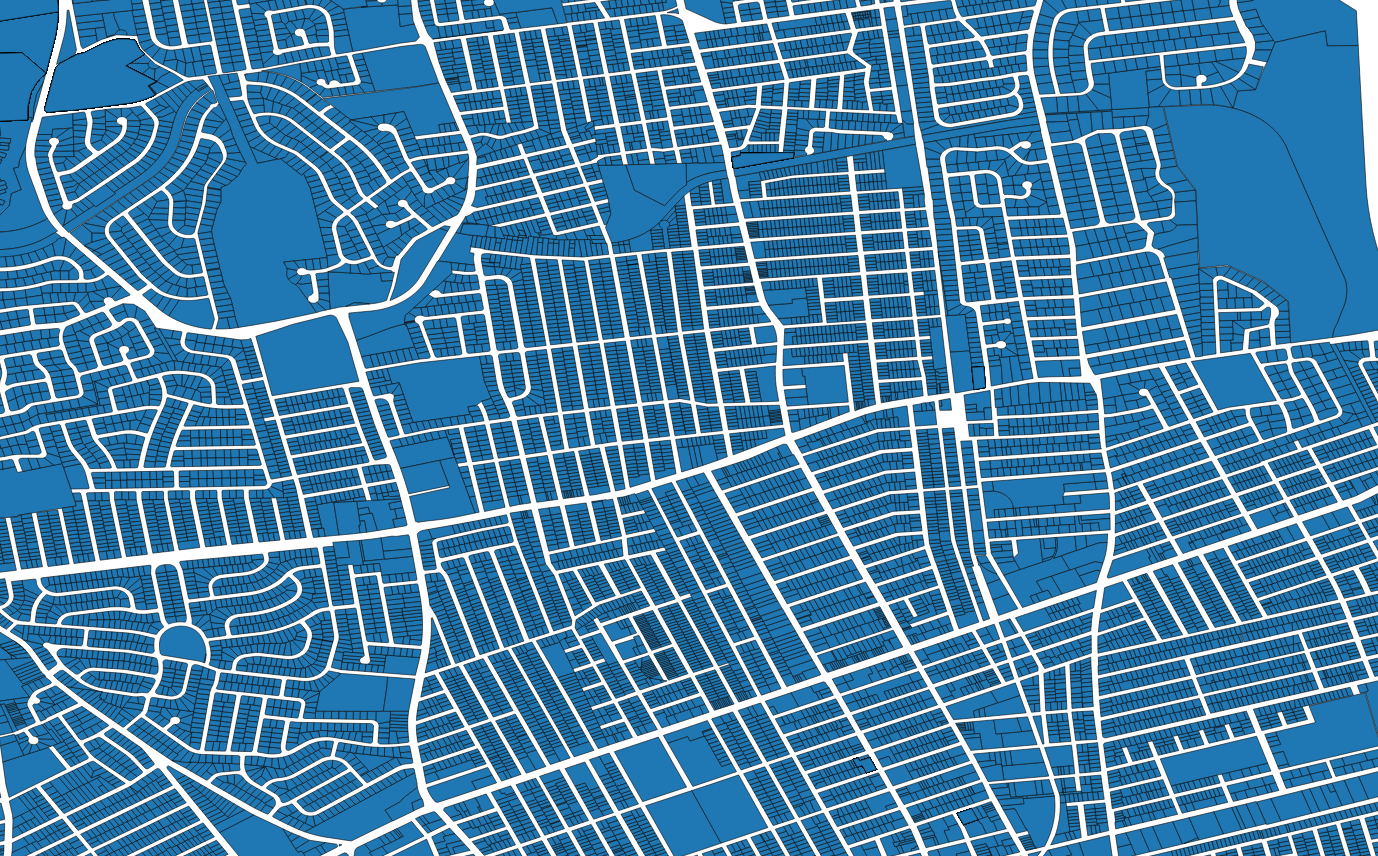
\includegraphics[width=0.9\textwidth]{parcel_dataset_images/neighborhood_level_lowres} % thrid figure itself
%				\caption{Zoomed-in View Highlighting Individual Parcels} 
				\footnotesize (c) Zoomed-in View Highlighting Individual Parcels
			\end{minipage}\hfill
		\caption{Multiple-scale view displaying the geospatial granularity accesible in the CoreLogics parcel data set.}
		\label{fig:parcelview}
	\end{figure}
%\end{conditionalfigure}

The information provided in the CoreLogics data set includes, among other information:

\begin{itemize}
	\item the `land use type' (e.g., hospital, quick service restuarant, etc.);
	\item the total land area of parcel;
	\item \hl{blah};
	\item \hl{blah};
	\item \hl{blah}.
\end{itemize}

In addition to sizing limitations on the application of wind turbines, some land-use types were considered incompatible with certain applications (e.g., residential land use types were considered unlikely to host utility-scale projects while `forest' and some agricultural land use types were considered to be incompatible with behind-the-meter applications). \hl{Although these land use type exclusions are subjective, a machine-learning approach will be considered for the final report in September}. Table~\ref{table:landusemap} in \ref{appendixa} shows all of the land use types considered in this analysis along with the eligible applications for that land use type and the assumed load pattern used with the land type. Load patterns are used to determine the value of the distributed generation for behind-the-meter applications under the VDER and NEM frameworks (see Section~\ref{btm_cons}).


% For turbine siting and sizing considerations, this analysis used similar considerations as the Distributed Generation Market Demand Model (dGen) \cite{sigrin_distributed_2016}. This includes
% images from the new data set

\subsection{Turbine Sizing}
\label{meth_sizing}

Wind turbines considered in this analysis for behind-the-meter, front-of-the-meter and utility-scale installations rely on mulitples of discrete turbine sizes as opposed to a continuous selection of wind turbines. Each turbine size is associated with a specific set of available hub heights. Furthermore, not all turbine sizes are available for all types of installations to reflect the fact that some turbines are simply too large to realistically be deployed behind-the-meter or too small to be deployed at the transmission-level (utility-scale). These hub-height and turbine sizes are shown below in Table~\ref{table:turbine_sizes} and are based on the original dGen turbine sizes. The assignment of certain sizes to specific applications is based on turbine classifications in \cite{sigrin_distributed_2016}. \hl{table classifications just placeholders!}

\hl{turbine size == rated capacity}

\begin{conditionaltable}[!htb]
\centering
  \begin{tabular}{lllSS|S|S|S|S}
    \toprule
      \multicolumn{5}{c}{} &
      \multicolumn{4}{c}{Hub Height (m)} \\
	\cmidrule{5-9}
        & {Application} & {Turbine Size Class} & {Turbine Size (kW)} & {20} & {30} & {40} & {50} & {80} \\
      \toprule
     	& Behind-the-meter 	& Small (Residential) 	& 2.5 		& \checkmark	& \checkmark	& \checkmark	& 				& 				\\
     	& Behind-the-meter 	& Small (Residential) 	& 5 		& 				& \checkmark	& \checkmark	& 				& 				\\
     	& Behind-the-meter 	& Small (Residential) 	& 10 		& 				& \checkmark	& \checkmark	& 				& 				\\
    	& Behind-the-meter 	& Small (Residential) 	& 20 		& 				& \checkmark	& \checkmark	& \checkmark	& 				\\
     	& Behind-the-meter	& Small (Commercial) 	& 50 		& 				& \checkmark	& \checkmark	& \checkmark	& 				\\
     	& Behind-the-meter 	& Small (Commercial) 	& 100 		& 				& 				& \checkmark	& \checkmark	& 				\\
     	& Front-of-the-meter & Midsize					& 250		& 	 			& 	 			& 	 			& \checkmark	& 				\\
     	& Front-of-the-meter & Midsize 					& 500 		& 	 			& 				& 				& \checkmark	& \checkmark	\\
    	& Front-of-the-meter & Midsize 					& 750		& 				& 				& 				& \checkmark	& \checkmark	\\
     	& Front-of-the-meter & Large 					& 1000		& 				& 				& 				& \checkmark	& \checkmark	\\
     	& Utility-scale 		& Large 					& 1500		& 	 			& 				& 				& 				& \checkmark	\\
    \bottomrule
  \end{tabular}
\caption{Wind Turbine Configurations Included in the Analysis Source: \citet{sigrin_distributed_2016}.}
\label{table:turbine_sizes}
\end{conditionaltable}

Any individual parcel may be subject to development constraints based on local siting conditions. In this analysis the primary siting constraints for wind turbine sizing are around available parcel size and canopy density and height similar to the basic dGen model assumptions \cite{sigrin_distributed_2016}. As there are over \hl{Forty Bajillion} parcels considered within the state of New York for this analysis, the available parcel size is simply taken to be the area of the given parcel less the footprint area of buildings within the parcel, assuming any are present. Considerations over the largest contiguous area available to develop a wind turbine are ignored as are considerations over the shape of the undeveloped space within a parcel. The total parcel area is given within the CoreLogics dataset \hl{while the building footprint area is determined from the Microsoft Blah Blah dataset}. Each of the turbine hub heights defined above in Table~\ref{table:turbine_sizes} are associated with a mimum available parcel size, outlined below in Table~\ref{table:hubheightparcel}.

Table B5 of \citet*{sigrin_distributed_2016} \hl{- is percent of highly-developed land considered in this analysis??}

\begin{conditionaltable}[!htb]
\centering
  \begin{tabular}{S|S}
    \toprule
	{Turbine Hub Height (m)} & {Minimum Parcel Size (acres)}\\
      \toprule
		\rowcolor{Gray}
		20 	& 0.50 \\
		30 	& 1.00 \\
		\rowcolor{Gray}
		40 	& 2.00 \\
		50 	& 3.00 \\
		\rowcolor{Gray}
		80 	& 4.00	\\
	\bottomrule
  \end{tabular}
\caption{Minimum Parcel Size Required for Each Available Hub Height. Source: \citet{sigrin_distributed_2016}.}
\label{table:hubheightparcel}
\end{conditionaltable}

In addition to available parcel sizes, tree canopy cover can also impact the maximum turbine size available to site a wind turbine within a given parcel. Similar to considerations outlined in \cite{sigrin_distributed_2016}, parcels with less than 25\% average canopy cover are defined as ``low canopy density'' areas and are not assigned any additional turbine sizing constraints. Parcels above this threshhold are considered``high canopy density'' areas and are subjected to additional constraints based on the average canopy cover height in the given parcel. Wind turbines in these ``high canopy density'' parcels must have a certain clearance above the tree cover, based on the size of the turbine rotor (Table~\ref{table:canopyclear}). Tree canopy density has been determined using a high-resolution (30-m by 30-m) grid of percentage of canopy cover included in the National Land Cover Data set 2011 (NLCD) \cite{jin_comprehensive_2013}. Average canopy cover height has been determined using the high-resolution (30-m by 30-m) National Biomass and Carbon Data set \cite{kellndorfer_nacp_2013}.

\begin{conditionaltable}[!htb]
\centering
    \pgfplotstabletypeset[column type = lcc, multicolumn names,
      col sep=comma,
	display columns/0/.style={fixed, fixed zerofill, precision=1, column name={Turbine Size (kW)}},
	display columns/1/.style={fixed, fixed zerofill, precision=1, column name={Approx. Rotor Radius (m)}},
	display columns/2/.style={fixed, fixed zerofill, precision=2, column name={Required Clearance (m)}},
	every head row/.style={
		before row=\toprule, 
		after row= \midrule},
	every last row/.style={
		after row=\bottomrule
		},
    ]{\canclear}
\caption{Canopy Clearance Required for Each Turbine Size (i.e., Rated Capacity). Source: \citet{sigrin_distributed_2016}.}
\label{table:canopyclear}
\end{conditionaltable}

\hl{need to explain all this canopy business better}

\subsection{Turbine Generation Characterization}
\label{meth_generation}

Wind generation in this analysis is a function of the available underlying resource, the wind speed at the corresponding hub height, and the power curve of the corresponding turbine. The hourly averge wind speeds at various hub heights for the typical meteorological year (TMY) at a medium resolution (20-km by 20-km) were provided in the AWS TruePower data set \cite{awst_3_2012}. These 20 km blocks are further resolved into 200m blocks using the methodology described in \cite[Appendix~B2]{sigrin_distributed_2016}. Wind speeds at hub heights not available in the AWS TruePower data set are calculated using wind speeds at available hub heights and a power-law for vertical adjustement described in \cite[Appendix~B2]{sigrin_distributed_2016}. Figure~\ref{fig:windspeeds} shows the \hl{average annual} wind speed at a \hl{resolution of 200m blocks} at a hub height of 80 meters for the state of New York. Generic power curves for four representative classes of wind turbines (small residential, small commercial, midsize and large) were developed based on a survey of actual turbines' normalized power curves as described in \cite[Appendix~B3]{sigrin_distributed_2016}. \hl{These power curves are to be updated \ldots}. Using wind speed data and assumed power curves for various wind turbine classes, hourly annual generation profiles can be created for each turbine at each location in the analysis.

\begin{conditionalfigure}[!htb]
  \centering
	  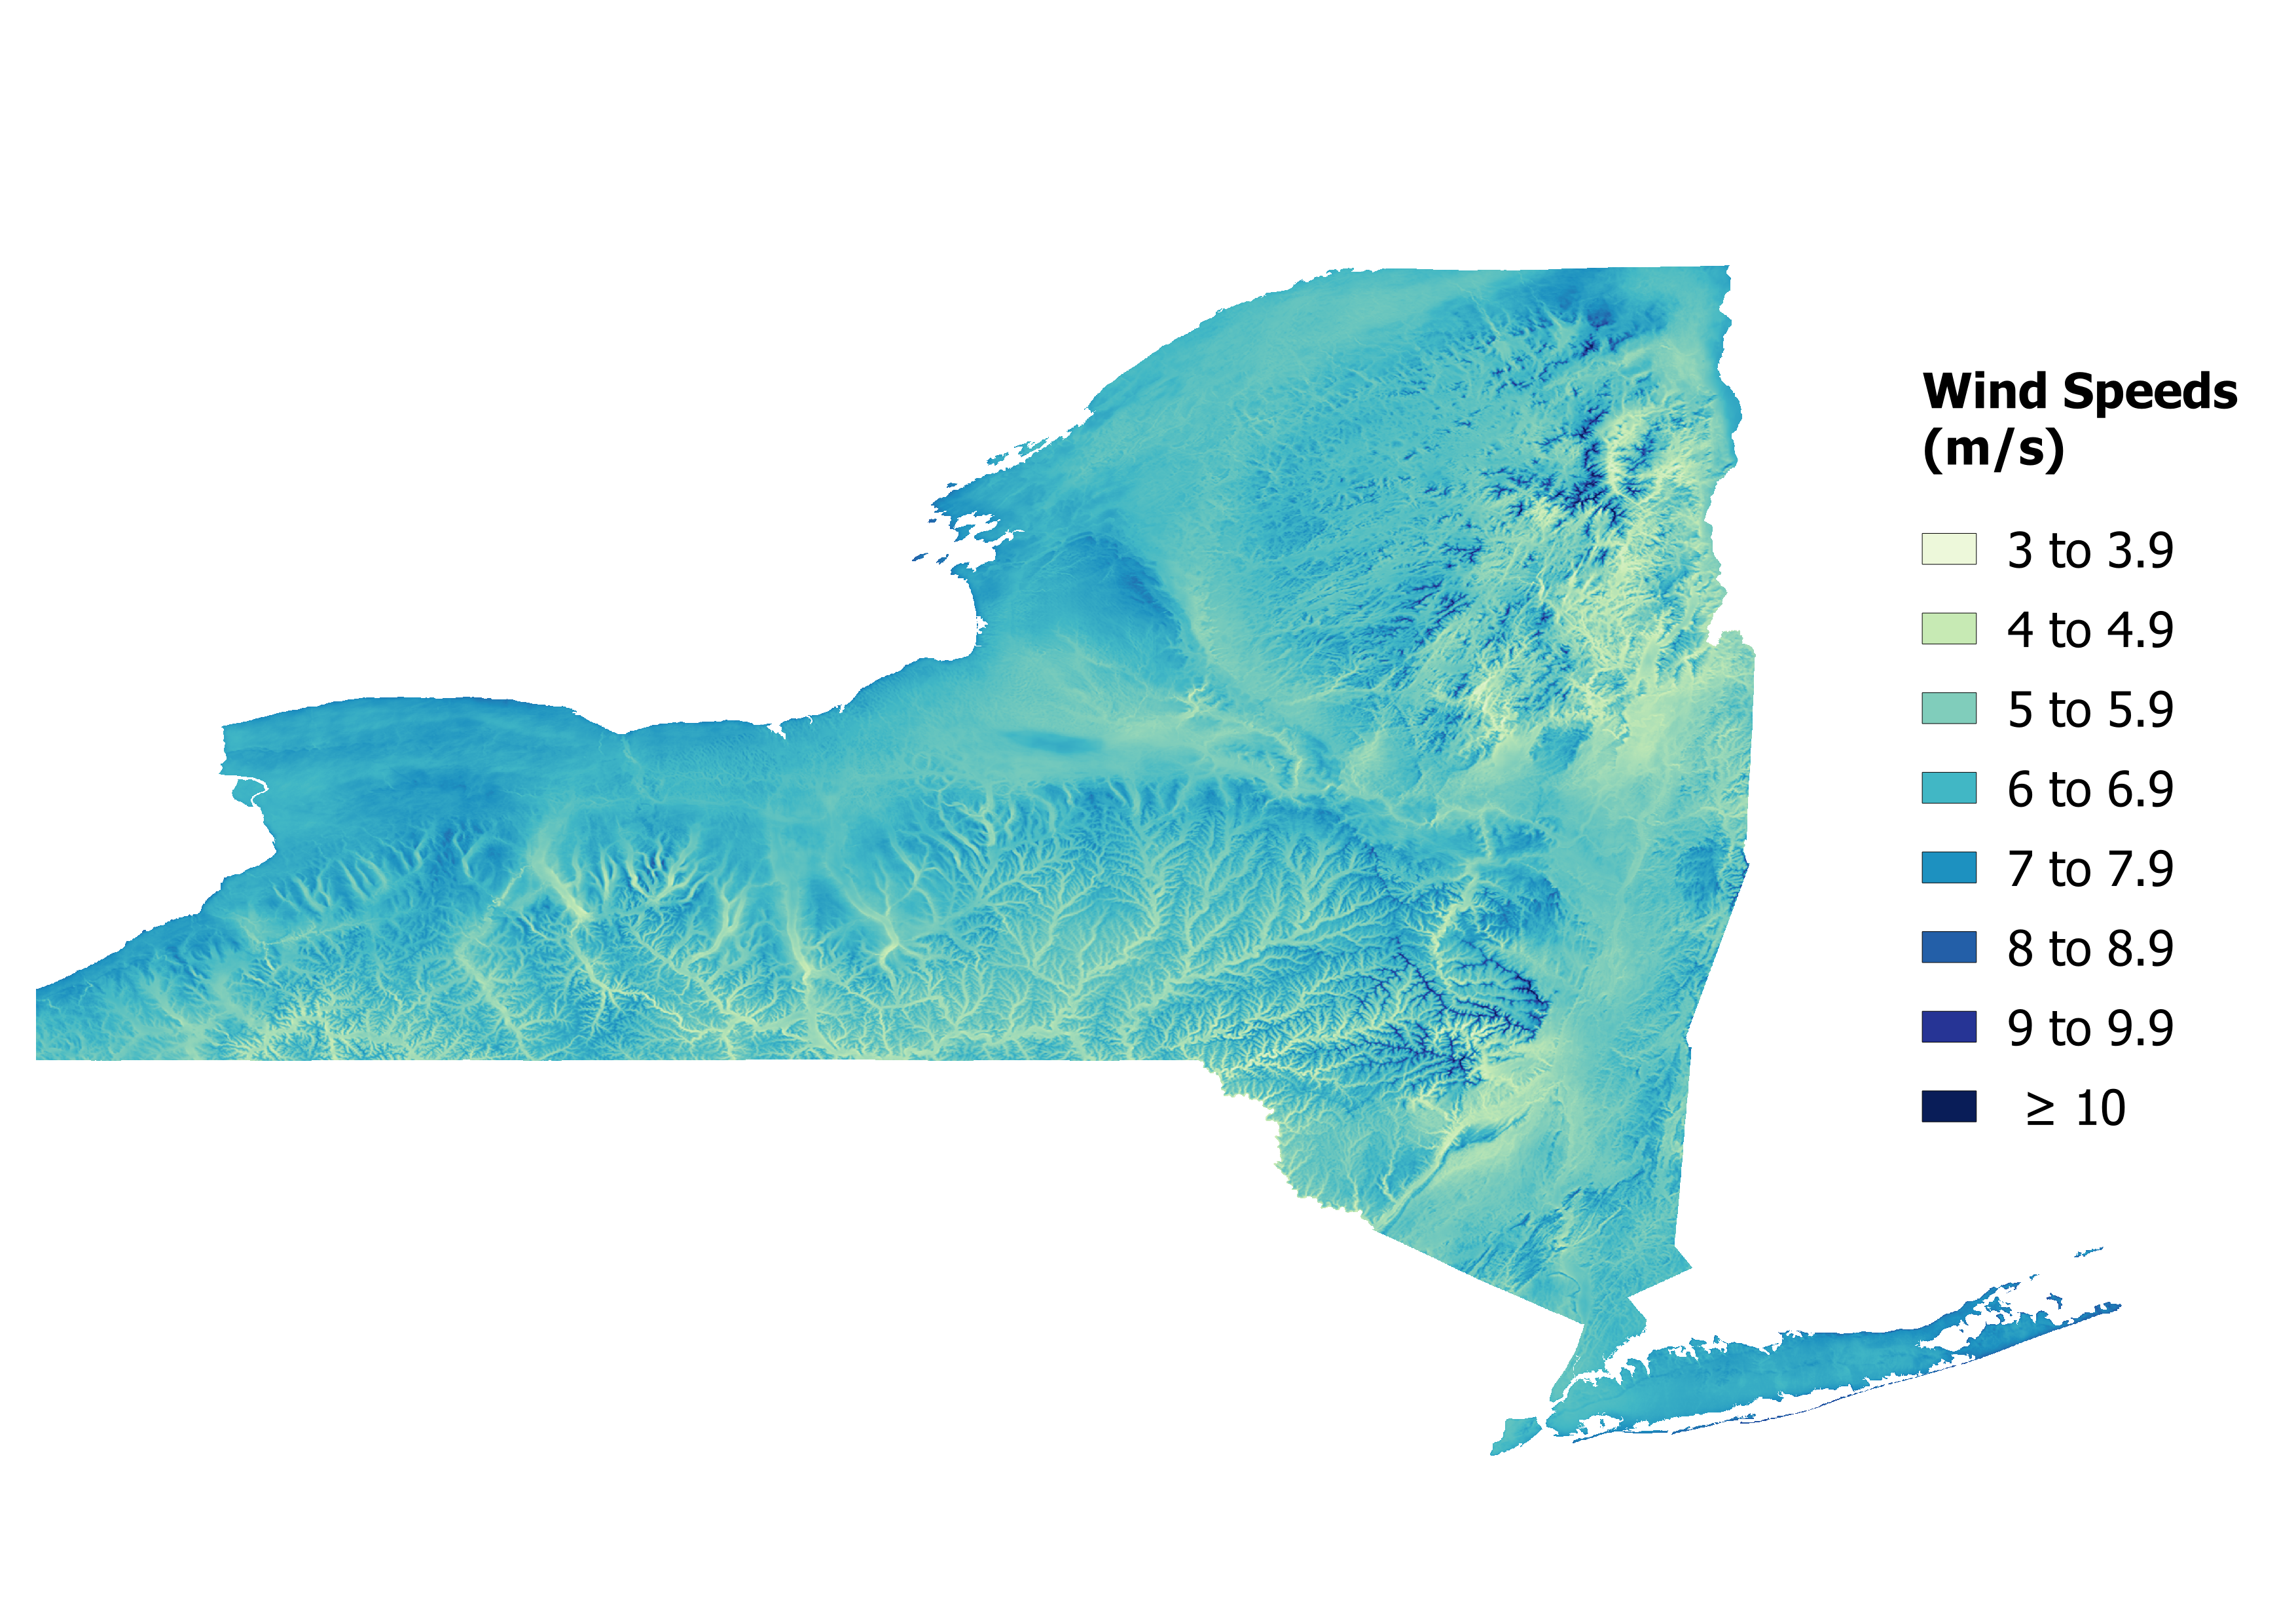
\includegraphics[width=.9\linewidth]{wind_speeds_at_80m_hub_height.png}
	  \caption{Average annual wind speeds at a hub height of 80m. Source: \citet{awst_3_2012}.}
	  \label{fig:windspeeds}
\end{conditionalfigure}

\vspace*{10mm}
\centerline{\large\textsc{Power curves for wind turbines here}}
\vspace*{10mm}

%% Difference between 'DER generation' and 'DER exports to the grid'??

\subsection{Load Zones and Utility Territories}
\label{meth_loc}
For this study all of the NYISO load zones and all of the larger utility territories were evaluated for their potential to site front-of-the-meter wind and the value of those exports to the grid. As municipal utilities are not required to offer VDER as a tariff/compensation mechanism,they were excluded from consideration. Figure ~\ref{fig:utilterr} shows the major utility territories in the state of New York. Figure ~\ref{fig:loadzones} shows the major NYISO load zones in the state of New York.\footnote{Shapefiles of the utility territories and NYISO Load Zones used in this analysis were obtained from \cite{government_of_new_york_nys_2020} and \cite{new_york_power_authority_nyiso_2014}, respectively.}


%% Note to self - fix maps to include municipal utility territory and merge con edison territory

\begin{conditionalfigure}[!htb]
  \centering
	  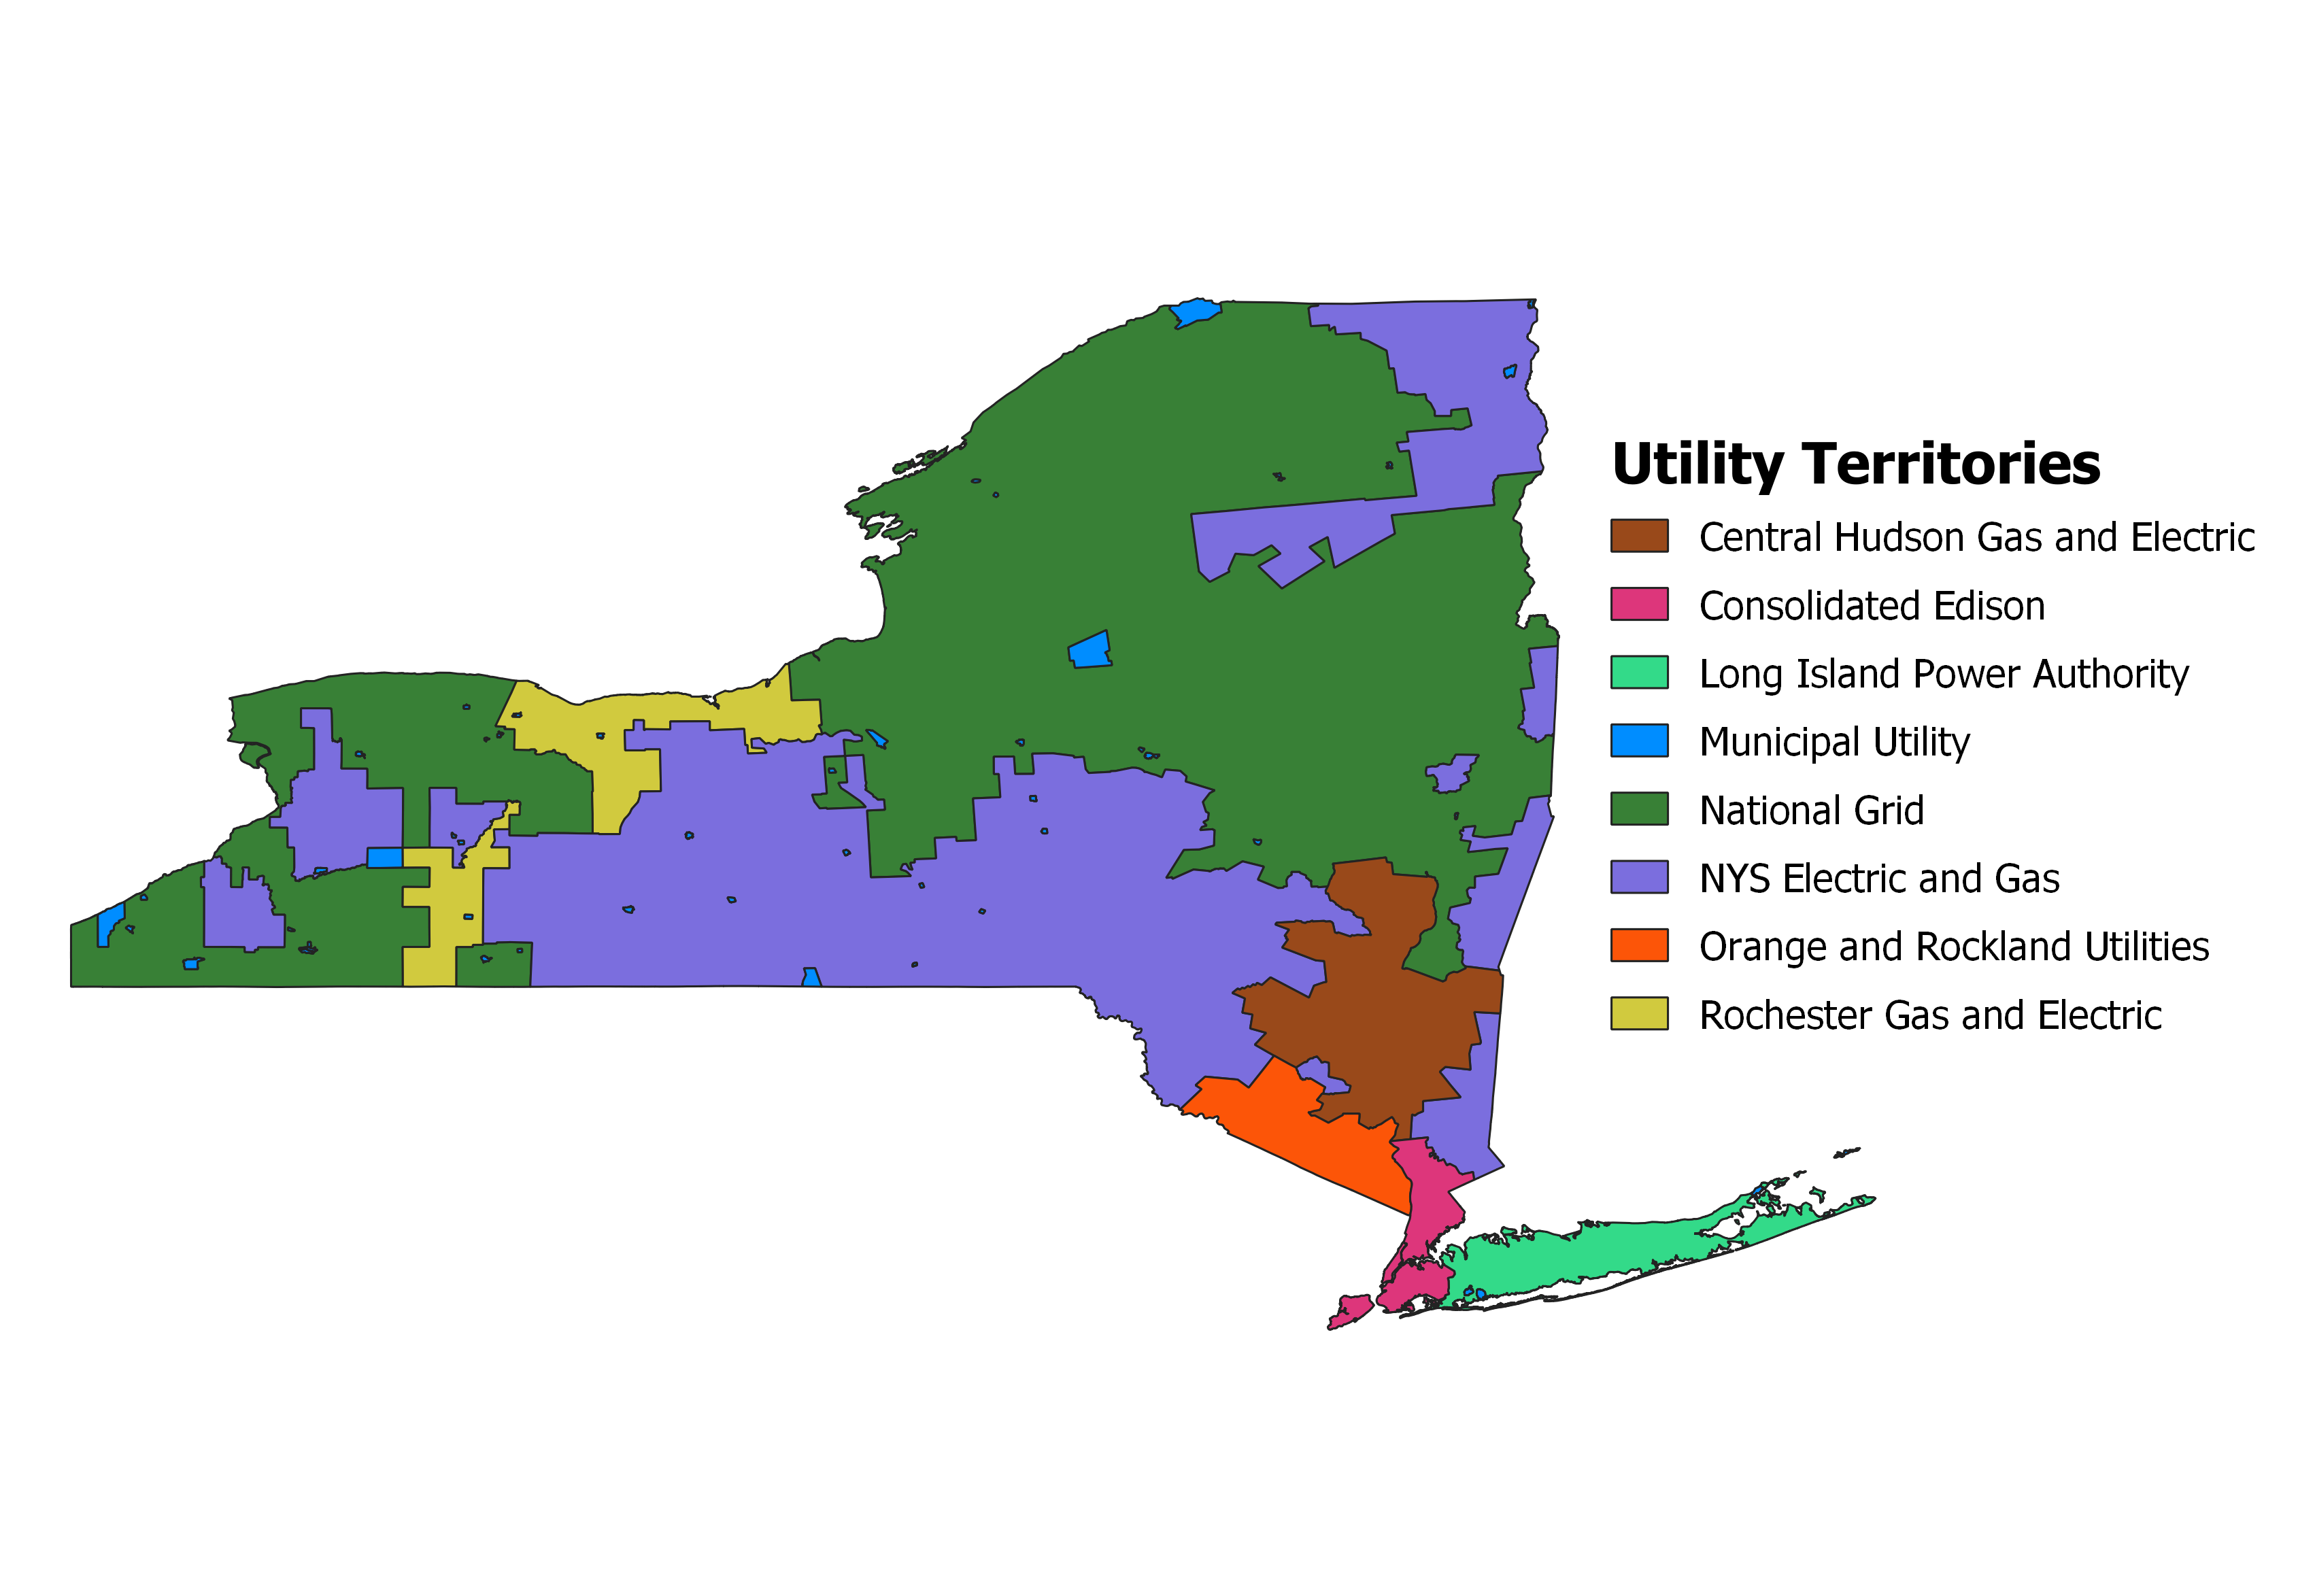
\includegraphics[width=.8\linewidth]{Utility_Territory_new.png}
	  \caption{Major New York Utility Territories, with Municipal Utilities}
	  \label{fig:utilterr}
\end{conditionalfigure}

\begin{conditionalfigure}[!htb]
  \centering
	  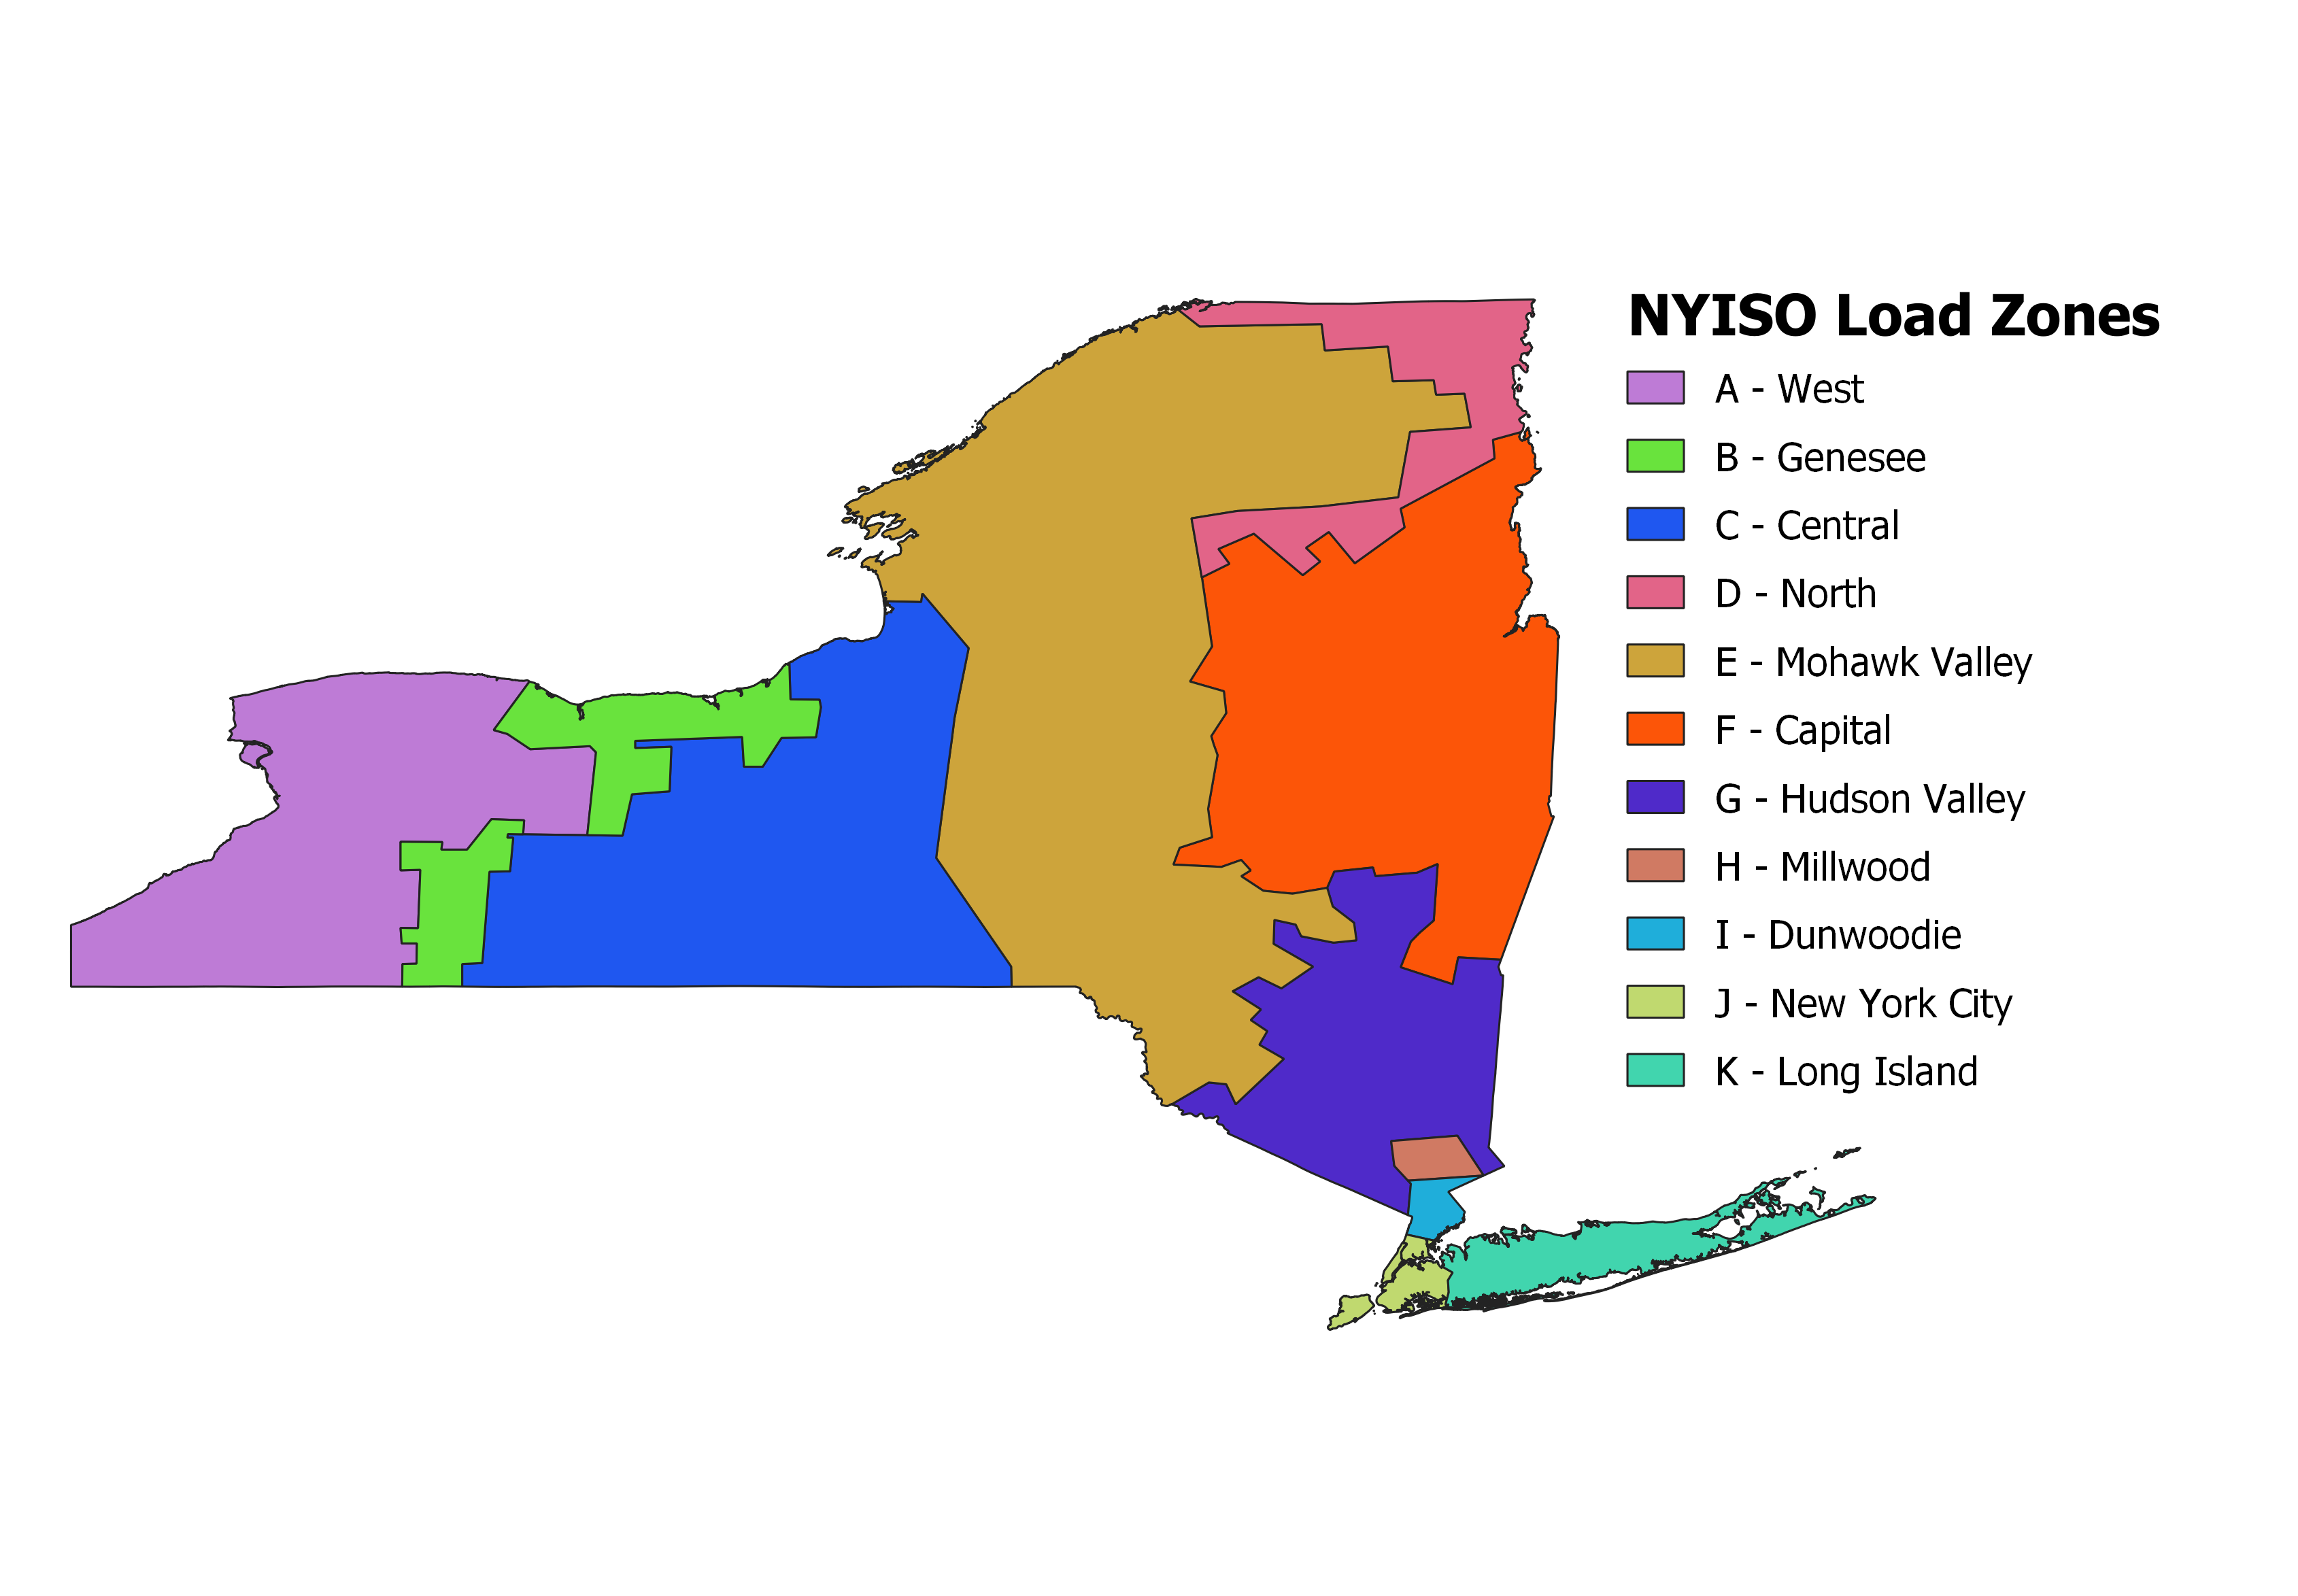
\includegraphics[width=.8\linewidth]{NYISO_Load_Zones_new.png}
	  \caption{NYISO Load Zones}
	  \label{fig:loadzones}
\end{conditionalfigure}

%\begin{figure}[h!]
%  \centering
%  \begin{subfigure}[b]{0.4\linewidth}
%    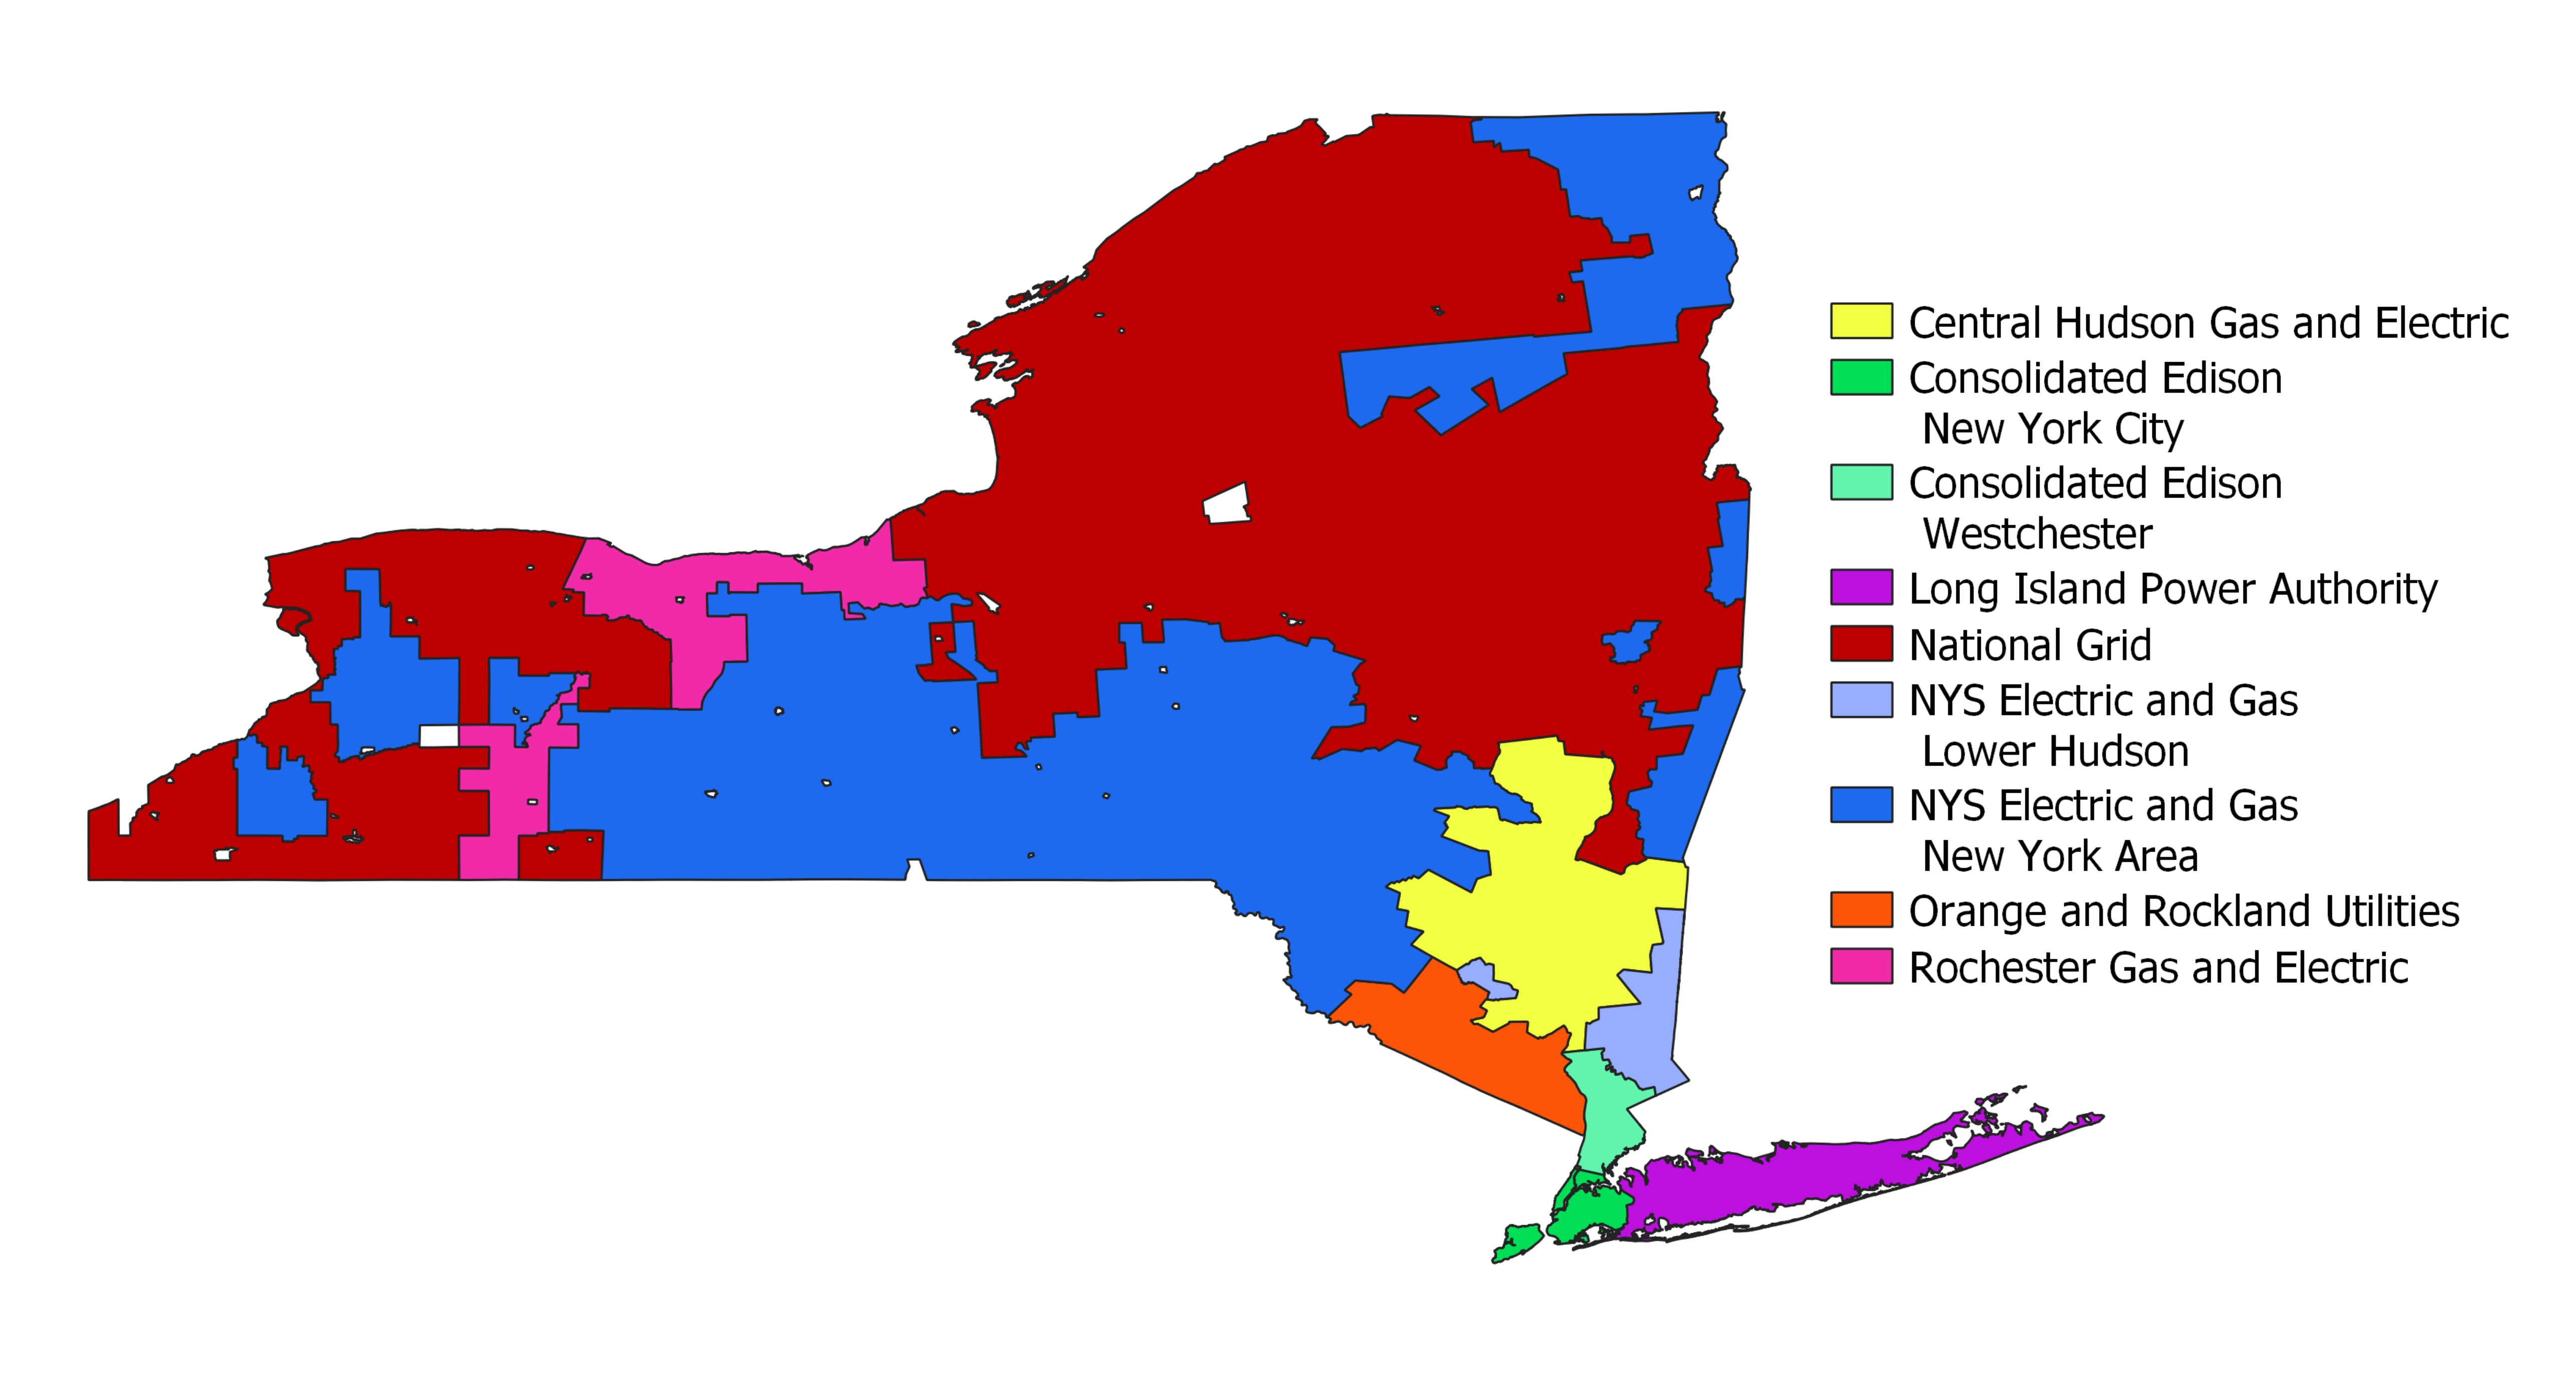
\includegraphics[width=\linewidth]{New_York_Utility_Territories_cropped.png}
%    \caption{Utility Territories.}
%  \end{subfigure}
%  \begin{subfigure}[b]{0.4\linewidth}
%    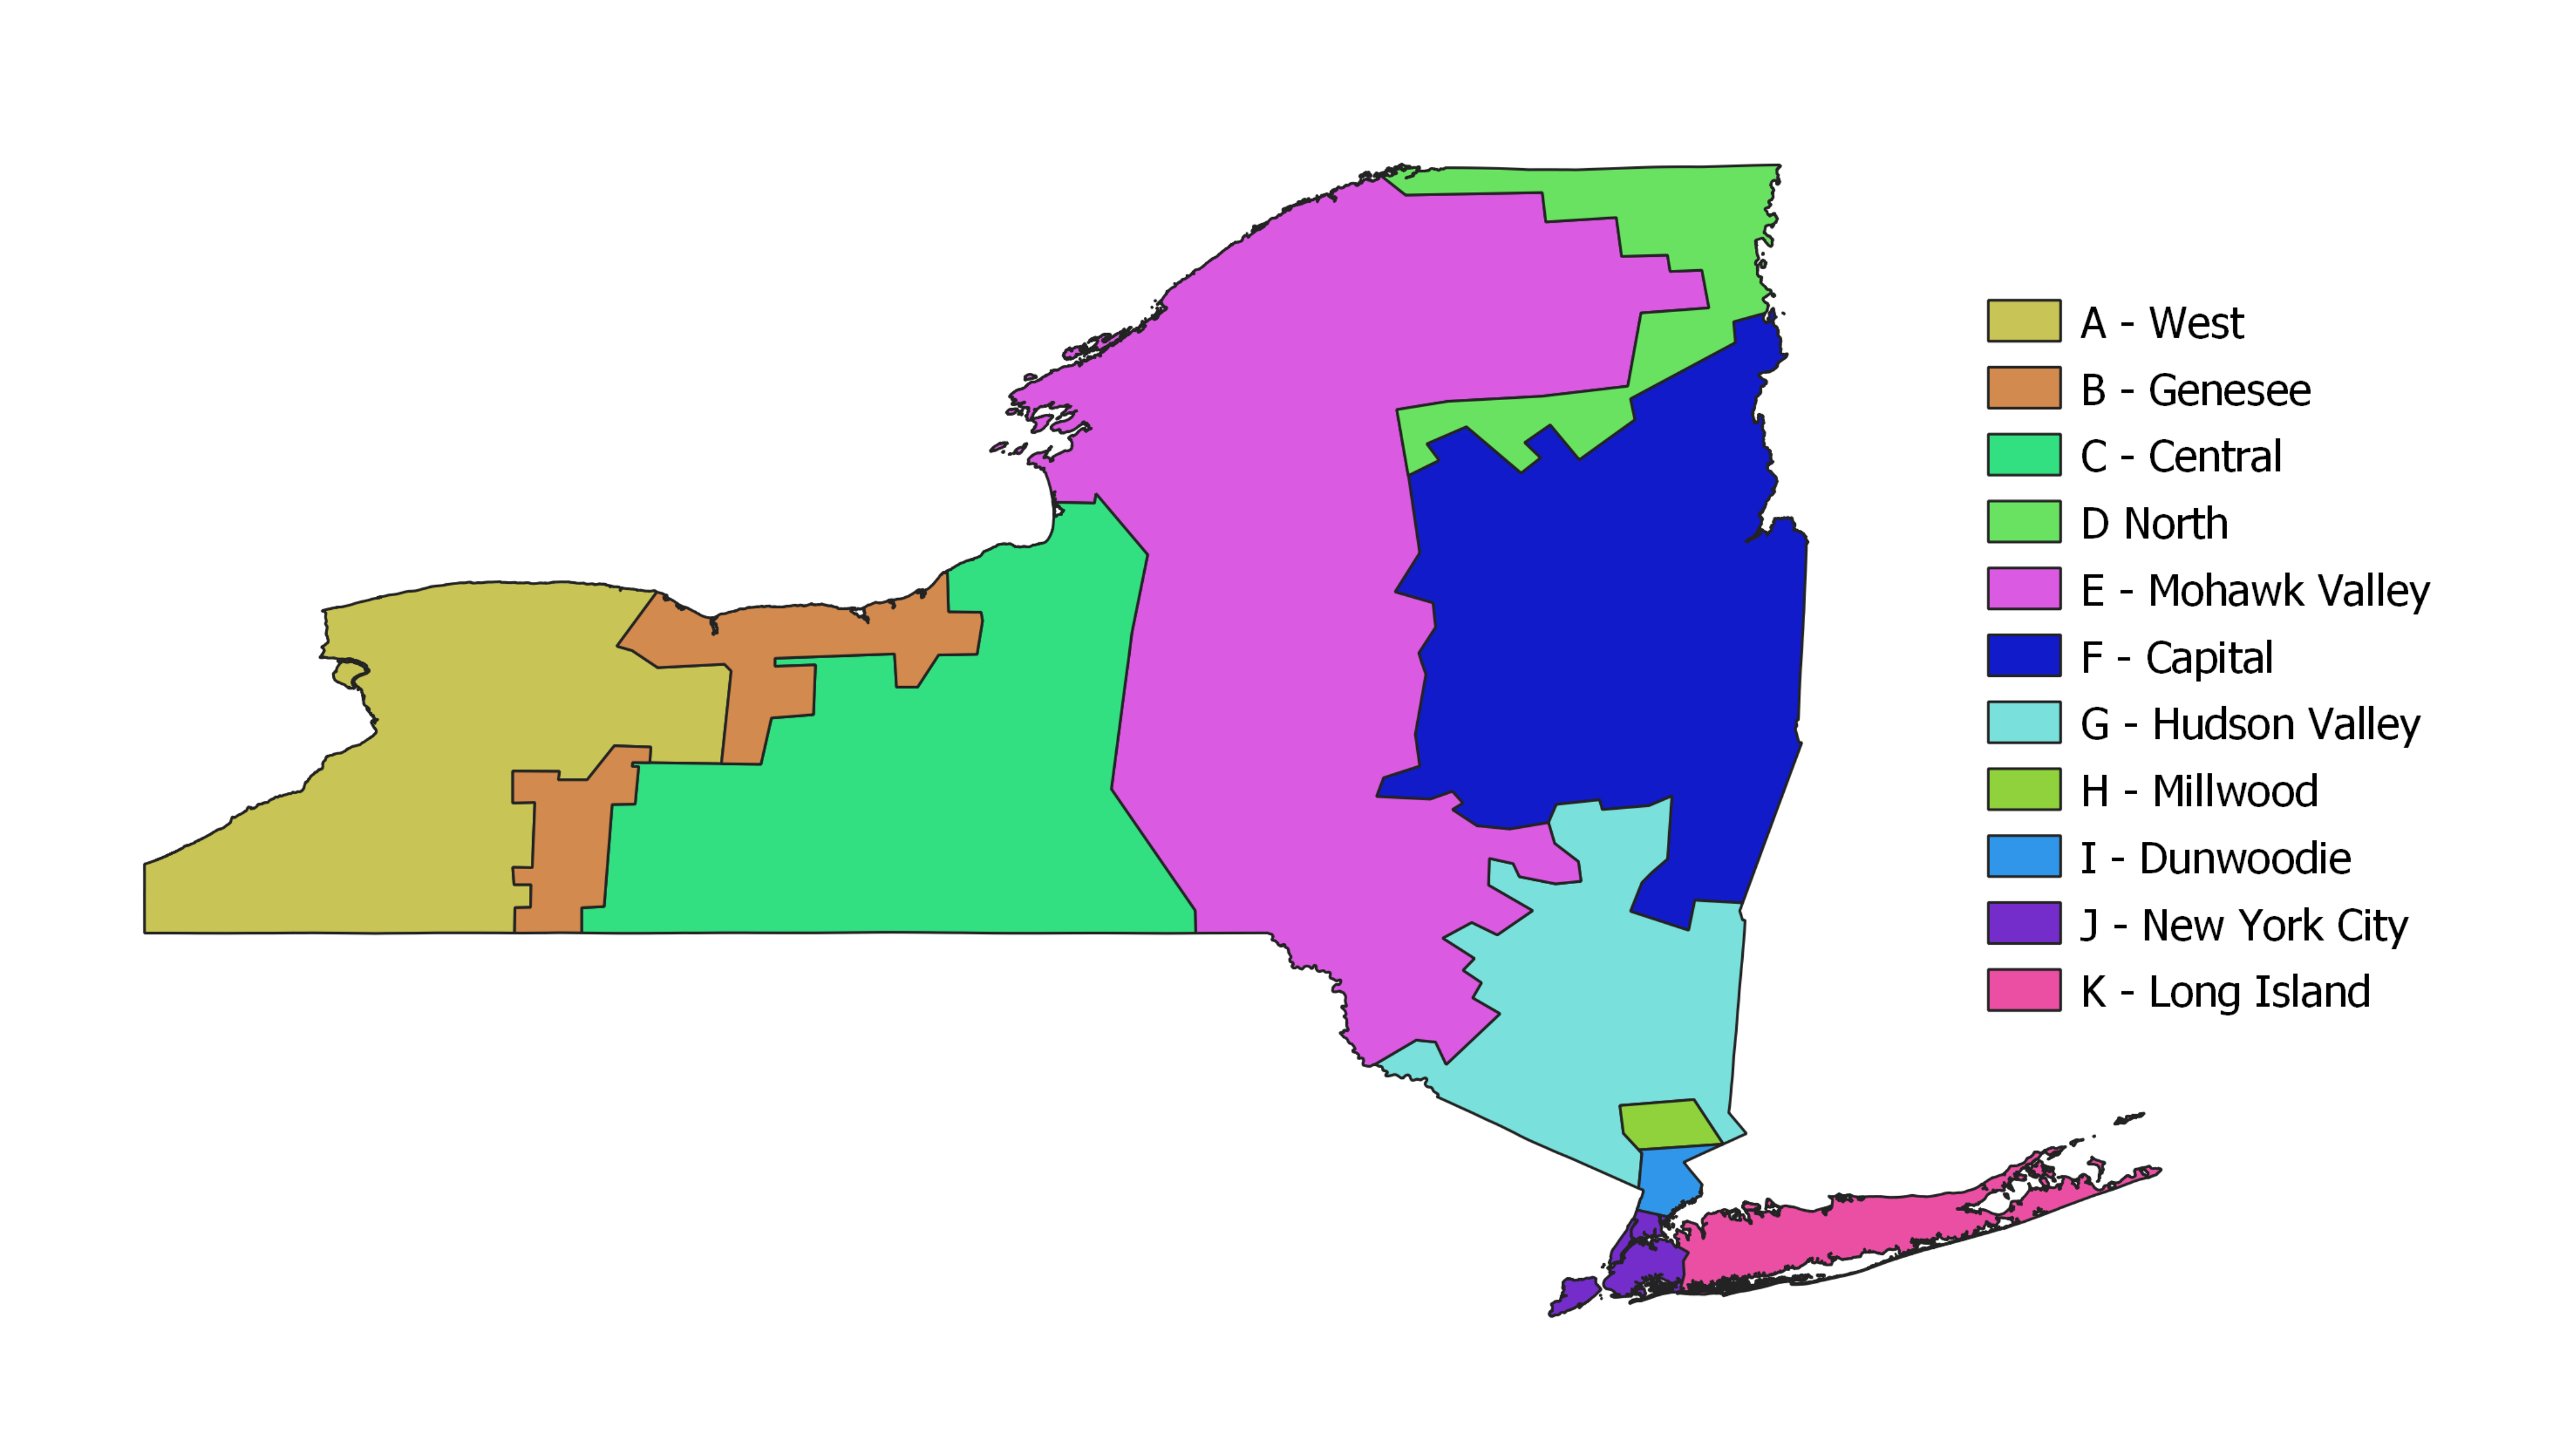
\includegraphics[width=\linewidth]{NYISO_Load_Zones_cropped.png}
%    \caption{Load Zones.}
%  \end{subfigure}
%  \caption{Major Utility Territories, Excluding Municipal Utilities, and NYISO Load Zones within the state of New York. \\ Source: \cite{government_of_new_york_nys_2020, new_york_power_authority_nyiso_2014}.}
%  \label{fig:utilterrandzones}
%\end{figure}

\subsection{Behind-the-meter Load and Net Energy Metering Considerations}
\label{btm_cons}

\vspace*{10mm}
\begin{centering}
\textsc{Address how BTM load and NEM were accounted for in the analysis}
\end{centering}
\vspace*{10mm}

\vspace*{10mm}
\begin{centering}
\textsc{Whole section needs heavy review for accuracy}
\end{centering}
\vspace*{10mm}

When determining the value of wind energy, behind-the-meter applications warrant two major additional considerations. 

First, behind-the-meter customers typically install distributed generation systems in order to minimize their electricity bill.\footnote{In other contexts distributed generation could be primarily installed for power reliability, but in this analysis for the state of New York we consider the primary metric for installing and sizing systems to be financial returns through electricity bill reductions.} \hl{This means customers will site systems not based on the largest system that could be sited on their property, but rather the system which minimizes their electricity bill.} Determining the optimal sizing for a system to reduce bills depends on three factors: 1) the customer's retail tariff rate; 2) the customer's load profile; and 3) the wind resources at the customer's property. The retail tariff rate for behind-the-meter applications was assigned from the Utility Rate Database (URDB) based on which utility territory the behind-the-meter parcel was located and to which load sector the parcel's land use type belonged (Residential, Commercial, Industrial, Agricultural) (see Table~\ref{table:landusemap} in Appendix~\ref{appendixa}) \cite{open_energy_information_utility_2020}. \hl{Table in Appendices of availabile tariff rates in New York by utility (at least those we considered) (might be good if we determined that distributed wind worked well for a particular customer class or tariff)?} The customer's load profile was determined based on \hl{blah data set for the overall load shape and the parcel area size to scale up the generic load shape to the appropriate magnitude}. Wind resource availability at the customer's site is determined as stated above in Section~\ref{meth_generation}.

Second, behind-the-meter generation can qualify for an alternative compensation mechanism known as Net Energy Metering (NEM). Under NEM, all customer exports are credited at the retail tariff rate and can be used to offset consumption within the same (or future) billing cycles. Under NEM, both self-consumed generation and exported generation are worth the retail tariff rate for the customer in question \cite{zinaman_grid-connected_2017}.\footnote{This valuation can be complicated by retail tariff rates whose charges vary throughout time (e.g., under time-of-use rates).} This is different than under the VDER framework wherein exports are valued at the 'Value Stack' (detailed below) but onsite consumption is valued at the customer's retail rate as under NEM. As customers with distributed generation are eligible for both NEM and VDER, this analysis attempted to quantify the value of behind-the-meter wind applications across the state under both compensation mechansisms. In most cases, one would expect that NEM would be a more generous compensation mechanism than VDER as retail tariff rates are designed to recover both variable and fixed costs associated with delivering power that customer exports cannot reasonably offset. This means that customers under NEM would most often receive compensation in excess of the actual value of their exports, which is more accurately determined under the VDER framework.\footnote{The authors are not suggesting that NEM is somehow an illegitimate compensation mechanism simply because it values distributed generation exports in excess of their real-time value. NEM has been successfully used throughout the United States and around the world as a tool to foster distributed generation markets in accordance with broader policy objectives that transcend a purely power-sector focused perspective.} In some locations and at specific times, however, it is possible that the VDER framework is more generous than the NEM framework as retail tariff rates (and therefore NEM compensation rates) typically are set to recover utility costs on an average, annual basis across a utility's entire territory. As discussed in Section~\ref{intro_vder}, this geospatial and temporal averaging provides little information (or incentive) to customers and developers to change their demand patterns, distributed generation operating patterns or deployment patterns to maximize value to the power system.

